\section{The Carbon Cycle}
\label{sec:carbon-cycle}

\newcommand{\COtwo}{CO\textsubscript{2}\ }  % Carbon Dioxide

\subsection{Fast and Slow Carbon Cycle}
\label{sec:fast-slow-carbon}

\begin{itemize}
    \item \textbf{Fast Carbon Cycle:} This is the flow of carbon from a reservoir or store to another where each cycle 
    takes about 10s of years. This tends to include the atmopshere, biosphere, soils and upper ocean. These stores are
    relatively small. 

    Anthropogenic changes in the stores are relatively small when compared to natural cycles, but still disturb the 
    natural balance of the cycle

    \item \textbf{Slow Carbon Cycle:} This is the flow of carbon from a reservoir or store to another where each cycle
    takes 100,000s of years. This tends to include the deep ocean and geological sediments (e.g. fossil fuel reseroirs
    or carbonate rocks like limestone). These stores are relatively large.
\end{itemize}

\subsection{Atmospheric Carbon Dioxide Concentrations, Emissions and Uptake}
\COtwo concentration is something that has changed over time due to natural and anthropogenic factors. Concentrations
are higher today than they have been at any point in the last 400,000 years. Over the last 1000 years up until 1750 (the
start of the industrial revolution) \COtwo concentrations were relatively stable at $\sim$285ppm. Since then they have
increased to the current level of $\sim$415ppm. 

Over this period, \COtwo has been the largest contributor to the total anthropogenic radiative forcing. This is a result
of the increase in \COtwo concentration in the atmosphere, its strong absorption peak at 15\textmu m and its long 
atmospheric lifetime.\\

Anthropogenic emissions of \COtwo are mainly due to the burning of fossil fuels and cement production. We can combine 
the net increase in \COtwo concentration in the atmosphere by considering the emissions and uptake of \COtwo in the 
three main sinks: the atmosphere, the ocean and the land biosphere. Furthermore, from this we can also consider the 
\textbf{airborne fraction} of \COtwo emissions (the fraction of emissions that remain in the atmosphere).

Research suggests that the land biosphere and ocean's ability to absorb \COtwo has increased over time, more than 
doubling since 1960. Without this, atmospheric concentrations of \COtwo would be even higher than they are today.

Over the past decade, of the $\sim$40 Gt\COtwo emitted each year, 46\% has remained in the atmosphere, 31\% has been
absorbed by the land biosphere and 23\% has been absorbed by the ocean.\\

\subsection{The Terrestrial Carbon Cycle}
\label{sec:terrestrial-carbon-cycle}

\subsubsection{Photosynthesis and Respiration}
\label{sec:photosynthesis_respiration}

Photosynthesis and respiration are the two main processes that control the exchange of \COtwo between the atmosphere and
the land biosphere. Photosynthesis \textit{removes} \COtwo from the atmosphere and is energy intensive and respiration
\textit{adds} \COtwo to it releasing energy.

Plants do not absorb all light equally when photosynthesising (hence them not being black). They are most sensitive
between 400-700nm. The absorption of light is used to drive the \textbf{Photosynthetically Active Radiation} (PAR): this
is the integral of the graph seen in figure \ref{fig:PAR_spectrum}. In said figure we can see a dip around the 550nm
region, which is green colour light, hence why plants are green. \\

\begin{figure}[h]
    \centering
    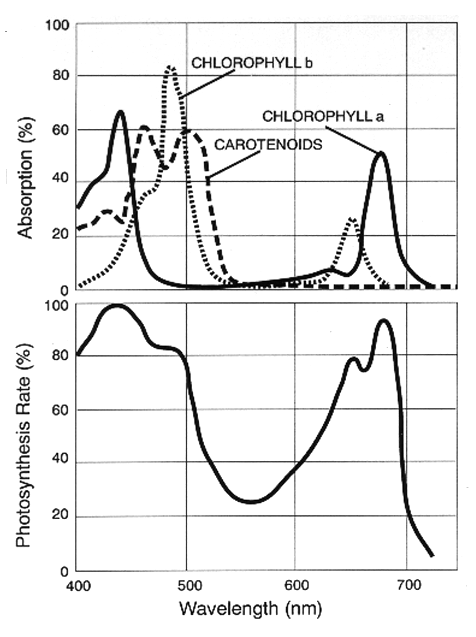
\includegraphics[width=0.5\textwidth]{figures/PAR_spectrum.png}
    \caption{The PAR Action Spectrum}
    \label{fig:PAR_spectrum}
\end{figure}

We can also define the productivity of an ecosystem with the \textbf{Gross Primary Productivity} (GPP) and the \textbf{Net
Primary Productivity} (NPP). GPP is the total amount of carbon fixed by photosynthesis in an ecosystem per unit time,
whereas NPP is the GPP minus the amount of carbon released by respiration i.e. $NPP = GPP - R$.

Around 50\% of the GPP is used for respiration, the other 50\% is used for growth.

\subsubsection{The Terrestrial Biosphere as a Carbon Source and Sink}
\label{sec:terrestrial-carbon-source-sink}

As noted in section \ref{sec:carbon-cycle}, the terrestrial biosphere is a sink for \COtwo, both from natural and
anthropogenic origin. Natural variability of the terrestrial biosphere occurs and can perturb the magnitude of this
sink. 

However, anthropogenic activity has a significant impact. Indeed, land use and change through deforestation and some
agricultural practices have resulted in the terrestrial biosphere becoming a net source of \COtwo in some regions
(e.g. the tropics). On the contrary, in other regions this is in fact the opposite, where afforestation and reforestation
have resulted in the terrestrial biosphere becoming a net sink of \COtwo and some regions even have net negative land
carbon emissions.

It is important the permanence of the carbon sink is considered when thinking about the influence of the terrestrial
biosphere on atmospheric \COtwo concentrations. For example, wildfires can perturb concentrations, but vegetation
tends to regrow and reabsorb the \COtwo released, meaning this is a transitory effect.

\subsubsection{Climate-Carbon Feedbacks}
\label{sec:climate-carbon-feedbacks}

Both photosynthesis and respiration are temperature dependent. As such changes to the climate will perturb the terrestrial
carbon cycle and therefore the atmospheric \COtwo concentration. Some of these feedbacks follow:

\begin{itemize}
    \item `Greening' of the Earth due to the \textbf{CO\textsubscript{2} Fertilisation Effect}: This is the increase in
    photosynthesis due to the increase in \COtwo concentration in the atmosphere. This is a negative feedback as the
    increase in photosynthesis will result in a decrease in atmospheric \COtwo concentration, which will in turn result
    in a decrease in photosynthesis. This enhances the land carbon sink.
    \item Relaxation on factors limiting plant growth - water, sunlight availability and temperature.
    \item Increase in respiration due to the increase in temperature. This is a positive feedback as the increase in
    respiration will result in an increase in atmospheric \COtwo concentration, which will in turn result in an increase
    in temperature which leads to even more respiration. This limitex the land carbon sink.
\end{itemize}

The impact of these is non-trivial and is still an area of active research.

\subsection{The Oceanic Carbon Cycle}
\label{sec:oceanic-carbon-cycle}

The ocean is a large carbon sink for atmospheric \COtwo. It takes up \COtwo through the dissolution of \COtwo in the
surface ocean and transforms it into \textbf{Dissolved Inorganic Carbon} (DIC). We can define DIC as:

\begin{align}
\text{DIC} &= \text{Dissolved Carbon Dioxide} + \text{Carbonic Acid} + \text{Bicarbonate} + \text{Carbonate} \nonumber \\
\text{DIC} &= \text{CO\textsubscript{2 (aq)}} + \text{H\textsubscript{2}CO\textsubscript{3}} 
+ \text{HCO\textsubscript{3}\textsuperscript{-}} + \text{CO\textsubscript{3}\textsuperscript{2-}} \nonumber
\end{align}


As we can expect, DIC has increased over the last few decades due to the increase in anthropogenic \COtwo emissions.
As per teh equation above we can see that this increase in DIC leads to a decrease in pH, i.e. ocean adification. This 
is partially buffered but oceanic adification is still a an occurrence and therefore a concern.

\subsubsection{Controls on Oceanic Carbon Uptake}
\label{sec:controls-oceanic-carbon-uptake}

How much the oceans are able to absorbe \COtwo is dependent on two main factors: atmospheric \COtwo concentration and
oceanic temperature:
\begin{itemize}
    \item Oceans are able to absorb more \COtwo as DIC when atmospheric \COtwo concentration is higher. However, the 
    rise between atmospheric \COtwo concentration and DIC is not linear, meaning the oceans' ability to keep absorbing
    \COtwo as concentrations increase more and more is reducing.
    \item Oceans are able to absorb more \COtwo as DIC when oceanic temperature is lower. This is because the solubility
    of \COtwo in water is higher at lower temperatures. It therefore follows that increasing oceanic temperature reduces
    the oceans' ability to act as carbon sinks.
\end{itemize}

\subsubsection{The Ocean Biological Carbon Pump}
\label{sec:ocean-biological-carbon-pump}

This is the process by which carbon is transported from the surface ocean to the deep ocean. It is a biological process
where the transformation of DIC into organic carbon occurs through photosynthesis of marine plants and phytoplankton. 
These living organisms then die and sink to the deap ocean. During this process, some of the organic carbon will decompose
and be released back into the ocean as DIC. However, some of it will be buried in the deep ocean, which is a carbon sink.

The remineralisation depth, or the depth at which 63\% of the organic carbon has been remineralised determines the time 
interval until the carbon is released back into the atmosphere. A shallower depth will reduce the capacity fo the ocean
to draw down anthropogenic carbon emissions.

